
\section{Sistemi interconnessi - esteso}
È possibile suddividere un sistema comunque complesso, composto da più
sottosistemi che interagiscono tra loro.
Al fine di formalizzare correttamente i sistema interconnessi si presentano i
tre blocchi principali.

Il primo è il blocco sistema, rappresenta il modello di un sistema, disegnato
mediante un rettangolo, con le frecce in ingresso e in uscita si indicano le
variabili di ingresso e uscita.
$$
Y_f(s) = W(s)U(s)
$$
\begin{figure}[h]
\centering
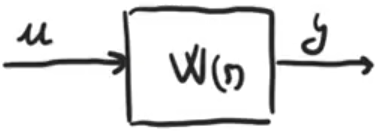
\includegraphics[width=0.3\linewidth]{blocco_sistema}
\end{figure}

Il secondo elemento è il nodo diramatore, ha un ingresso, poi con un punto
calcato si suddividono le uscite (nel dominio del tempo o di Laplace
$$
y_1(t) = y_2(t) = y_3(t) = u(t)
$$
\begin{figure}[h]
\centering
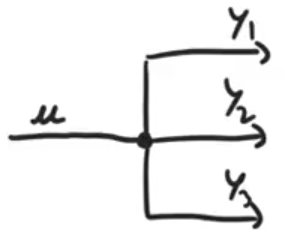
\includegraphics[width=0.3\linewidth]{blocco_nodo}
\end{figure}

\newpage
Il nodo sommatore invece, rappresentato mediante un cerchio o un quadrato
esegue somme o sottrazioni degli ingressi, fornendo una sola uscita
$$
y(t) = u_1(t) - u_2(t) + u_3(t)
$$
\begin{figure}[h]
 \centering
 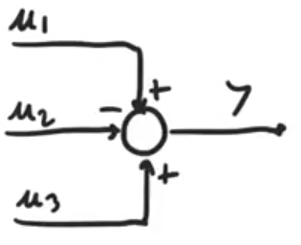
\includegraphics[width=0.3\linewidth]{blocco_sommatore}
\end{figure}

Per ottenere la rappresentazione di tutto il sistema è comodo operarne la sua
riduzione, per via algebrica o più comodamente per via grafica.
Le regole di riduzione si basano sulla presenza di tre connessioni canoniche,
in serie, in parallelo e in retroazione.

\subsection{Connessione in serie}
Due o più blocchi sono connessi in serie se l'ingresso del blocco
successivo coincide con l'uscita del precedente.
\begin{figure}[h]
\centering
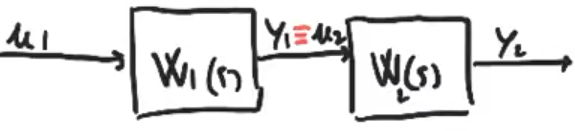
\includegraphics[width=\picwid]{blocchi_serie}
\end{figure}
Dal punto di vista sistemistico la serie può essere vista come un unico blocco
più grande con un'unica funzione di trasferimento $W(s)$ con ingresso $u$ e
uscita $y$.

Si ricava la riduzione, si presentano le relazioni algebriche dei due blocchi e
il vincolo topologico
$$\left\{\begin{aligned}
Y_1(s) &= W_1(s)U_1(s) \\
Y_2(s) &= W_2(s) U_2(s) \\
Y_1(s) &= U_2(s)
\end{aligned}\right.
\qquad
\begin{aligned}
Y(s) &= Y_2(s) = W_2(s)U_2(s) = W_2(s)Y_1(s) =\\
&=W_2(s)W_1(s)U_1(s) = W_2(s)W_1(s)U(s)
\end{aligned}$$
La funzione di trasferimento del blocco ridotto è dunque pari al prodotto delle
due funzioni di trasferimento dei sottosistemi.
Se il sistema è SISO la moltiplicazione è commutativa, non è vero per i sistemi
non SISO.

\newpage
\subsection{Connessione in parallelo}
Due o più sottosistemi sono connessi in parallelo se condividono lo stesso
ingresso, uscita di un nodo diramatore, e la loro uscita viene combinata in un
nodo sommatore.
\begin{figure}[h]
\centering
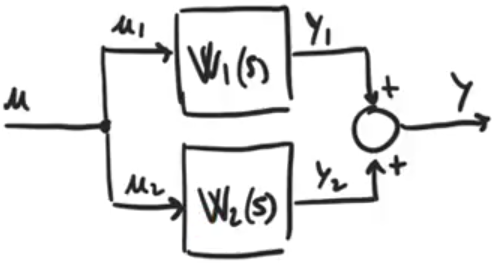
\includegraphics[width=\picwid]{blocchi_parallelo}
\end{figure}
Per ricavare l'unica funzione di trasferimento si procede in maniera analoga al
caso precedente, scrivendo le relazioni dei blocchi e dei due vincoli
sull'ingresso e l'uscita
$$
\left\{\begin{aligned}
Y_1(s) &= W_1(s) U_1(s) \\
Y_2(s) &= W_2(s) U_2(s) \\
U_1(s) &= U_2(s) = U(s) \\
Y(s) &= Y_1(s) + Y_2(s)
\end{aligned}\right.\qquad
\begin{aligned}
Y(s) & = Y_1(s) + Y_2(s) = W_1(s)U_1(s) + W_2(s) U_2(s) =\\
&=\left( W_1(s)+W_2(s)
\right) U(s)
\end{aligned}
$$
La funzione di trasferimento del blocco in parallelo è pari alla somma
algebrica delle rispettive funzioni di trasferimento dei sottosistemi.

\subsection{Connessione in retroazione}
Un sistema in retroazione è composto da due blocchi, il sistema $W_1$ che
genera l'uscita è chiamato \textit{catena di andata}, il blocco $W_2$ inferiore
prende il nome di \textit{catena di ritorno (o retroazione)} e chiude un anello
in cui ``girano'' le informazioni chiamato \textit{anello di retroazione}.
L'ingresso del sistema principale è dato dal confronto dell'ingresso $u$ di
riferimento e l'uscita $y_2$ del blocco di retroazione. Si può avere una
retroazione negativa o positiva a seconda del segno che compare nel blocco
sommatore in ingresso (quella in figura è negativa).

\begin{figure}[h]
\centering
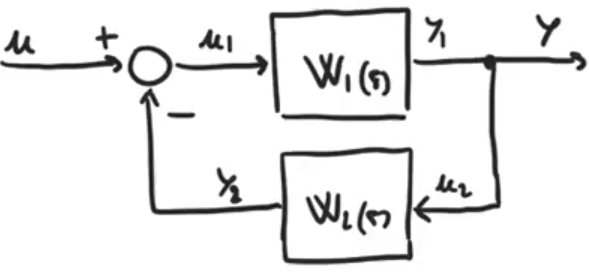
\includegraphics[width=\picwid]{blocchi_retroazione}
\end{figure}

Si analizzano le equazioni dei singoli blocchi e le due relazioni topologiche
$$
\left\{\begin{aligned}
Y_1(s) &= W_1(s) U_1(s) \\
Y_2(s) &= W_2(s) U_2(s) \\
U_1(s) &= U(s) - Y_2(s) \\
Y(s) &= U_2(s) = Y_1(s)
\end{aligned}\right.
$$

Sviluppando il sistema a partire dalla funzione in uscita si ricavano le due
funzioni di trasferimento per i sistemi in retroazione positiva e negativa
$$
\begin{aligned}
Y(s) & = W_1(s) U_1(s) = W_1(s) (U(s) - Y_2(s)) =\\
&=
W_1(s) (U(s) - W_2(s)U_2(s)) = W_1(s)(U(s)-W_2(s)Y(s)) \Rightarrow \\
&(1+W_1(s)W_2(s))Y(s) = W_1(s) U_1(s) \Rightarrow
Y(s) = \frac{W_1(s)}{1+W_1(s)W_2(s)}U(s)
\end{aligned}
$$
\begin{table}[h]
\centering
\begin{tabular}{c|c}
Retroazione negativa & Retroazione positiva \\
$W(s) = \frac{W_1(s)}{1+W_1(s)W_2(s)}$ &
$W(s) = \frac{W_1(s)}{1-W_1(s)W_2(s)}$
\end{tabular}
\end{table}

\subsubsection{Esempio non SISO}
Se il sistema non dovesse essere di tipo SISO come quello in esempio
$$
u=\begin{pmatrix}
u_1 \\ u_2
\end{pmatrix} \rightarrow
\begin{matrix}W(s)\\2\times2
\end{matrix}
\rightarrow y = \begin{pmatrix}
y_1 \\ y_2
\end{pmatrix}
$$
Sfruttando la sovrapposizione degli effetti si possono scomporre le uscite,
ogni termine può essere visto come la somma degli effetti di un singolo
ingresso alla volta, dunque per calcolare $y_1$ si studia la risposta ad $u_1$
quando $u_2$ è nulla e viceversa, poi si sommano i due contributi; analogamente
per $y_2$.
$$\left\{\begin{aligned}
Y_1 &= Y_1' + Y_1'' = W_{11}U_1 + W_{12}U_2\\
Y_2 & = Y_2' + Y_2'' = W_{21}U_1 + W_{22}U_2
\end{aligned}\right.$$

Dunque la $W(s)$ sarà
$$
W(s) = \begin{bmatrix}
W_{11}(s) & W_{12}(s) \\
W_{21}(s) & W_{22}(s)
\end{bmatrix}
$$
Da un punto di vista grafico saranno presenti quattro blocchi elementari
\begin{figure}[h]
\centering
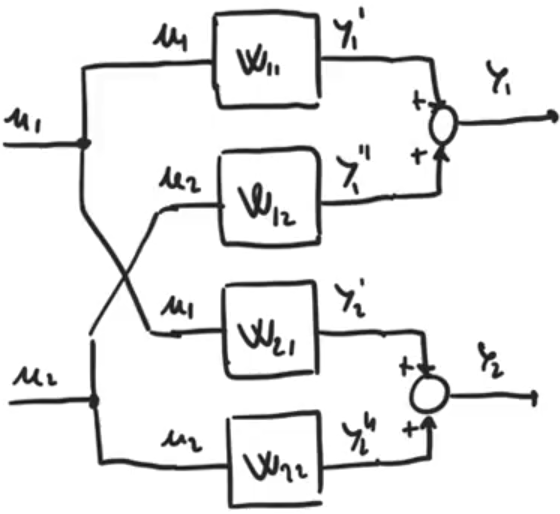
\includegraphics[width=\picwid]{blocchi_non_SISO}
\end{figure}

\subsection{Regole di riduzione}
Può capitare che in una rete complessa non sia chiaro quali blocchi siano in
serie o in parallelo, potrebbe essere necessario eseguire delle
\textit{manovre} di spostamento dei blocchi che coincidono ad operazioni
algebriche che devono lasciare però inalterata la funzione di trasferimento
complessiva.
Durante queste operazioni è molto probabile che si perda il senso fisico delle
operazioni, l'importante è non variare la funzione di trasferimento.

Si supponga di avere la seguente condizione, per qualche motivo si vuole
spostare il blocco $W(s)$ a monte del nodo sommatore, sarà equivalente al
sistema formato da due blocchi.
\begin{figure}[h]
\centering
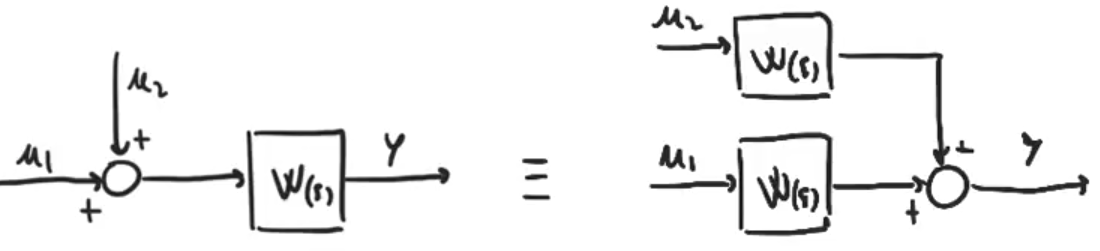
\includegraphics[width=0.7\linewidth]{blocchi_equivalenza_sommatore}
\end{figure}
Algebricamente si ottiene lo stesso risultato
$$
Y = W(U_1+U_2) \qquad \equiv \qquad Y= WU_1 + WU_2 = W(U_1+U_2)
$$
da un punto di vista fisico il sistema iniziale ha $n$ variabili di stato, il
secondo ha invece $2n$ variabili di stato, ma sono variabili ``fittizie'' e non
variabili fisiche.

Il caso duale è il seguente
\begin{figure}[h]
\centering
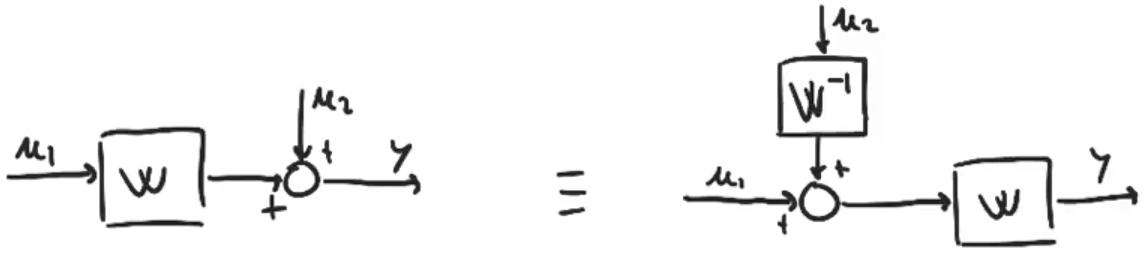
\includegraphics[width=0.7\linewidth]{blocchi_equivalenza_sommatore_a_valle}
\end{figure}
$$
Y = U_2 + WU_1 \qquad \equiv \qquad
Y = W(U_1 + W^{-1}U_2) = WU_1 + U_2
$$
I due sistemi sono ancora algebricamente equivalenti. Il sistema $W^{-1}$ ha un
ordine inverso rispetto al sistema $W$, se il sistema $W$ fosse un sistema
reale strettamente proprio, il sistema $W^{-1}$ diventerebbe improprio, il
numero di radici al numeratore sarebbe maggiore del numero di radici al
denominatore, dunque rappresenterebbe un sistema anticausale, non fisicamente
realizzabile.

\newpage
\subsubsection{Esempio di riduzione schema a blocchi}
Si riduca il seguente sistema
\begin{figure}[h]
\centering
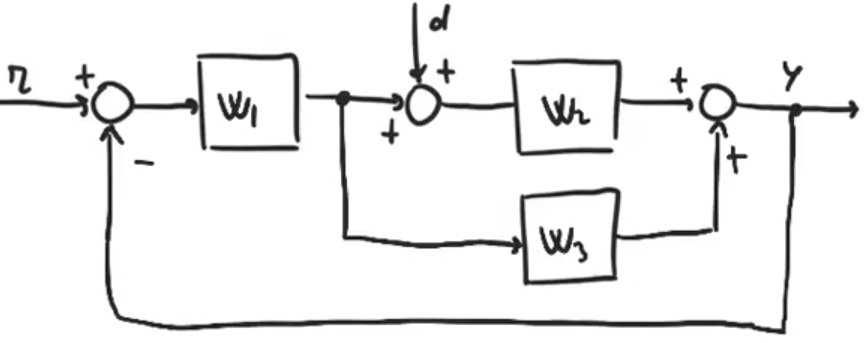
\includegraphics[width=0.7\linewidth]{blocchi_sistema_da_ridurre}
\end{figure}

Ha due ingressi $r$ e $d$ e un'uscita $y$, dunque la funzione di trasferimento
equivalente deve essere una matrice $(1\times2)$
$$
W(s) = \begin{bmatrix}
W_{y,r}(s) & W_{y,d}(s)
\end{bmatrix}
$$
Per ricavare il primo termine mediante il PSE si pone $d=0$, il nodo sommatore
in cui incide $d$ si elide, dunque i sottosistemi $W_2$ e $W_3$ si trovano ad
essere in parallelo, successivamente in serie al sistema $W_1$
\begin{figure}[h]
\centering
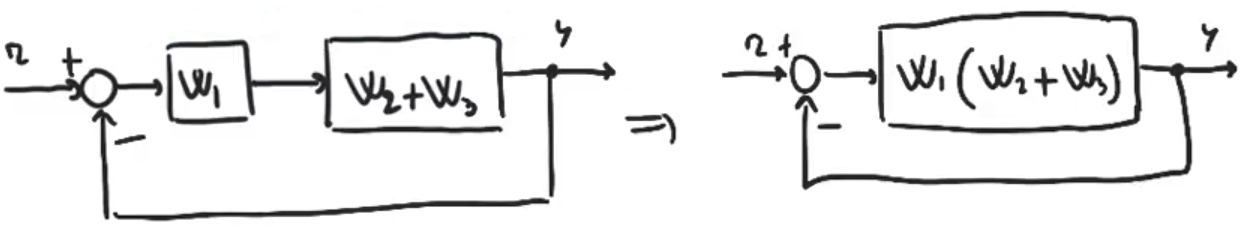
\includegraphics[width=0.8\linewidth]{blocchi_sistema_da_ridurre_Wr}
\end{figure}
In questo caso non c'è alcun blocco in retroazione, questo tipo di
collegamento coincide in realtà con una funzione di trasferimento unitaria, la
funzione di trasferimento complessiva, applicando la retroazione sarà dunque:
$$
W_{y,r}(s) = \frac{W_1(s)(W_2(s) + W_3(s))}{1 + W_1(s)(W_2(s) + W_3(s))}
$$
Per calcolare il secondo termine $W_{y,d}$ si deve annullare l'ingresso $r$ e
considerare solo quello $d$.

\newpage
\subsection{Analisi della stabilità di un sistema interconnesso}
\subsubsection{Sistemi in serie}
Si considerino due sistemi in serie $S_1$ ed $S_2$, si supponga di conoscere i
modelli ISU dei due sistemi
$$
\begin{aligned}
S_1 &: \left\{\begin{aligned}
\dot{x}_1 & = A_1x_1 + B_1u_1\\
y_1 &= C_1 x_1 + D_1u_1
\end{aligned}\right. \\
S_2 & : \left\{\begin{aligned}
\dot{x}_2 & = A_2x_2 + B_2u_2\\
y_2 &= C_2 x_2 + D_2u_2
\end{aligned}\right. \\
\text{Vincoli} &: \left\{\begin{aligned}
u&=u_1\\
y&=y_2\\
u_2 &=y_1
\end{aligned}\right.
\end{aligned}
$$
Si vuole studiare la stabilità dell'intero sistema dunque si può pensare di
aggregare le variabili di stato in un unico vettore, lo stato dell'intero
sistema è l'aggregazione dei due sottosistemi, si sostituiscono i termini
usando i vincoli
$$
x = \begin{pmatrix}
x_1 \\ x_2
\end{pmatrix}\qquad
\left\{\begin{aligned}
\dot{x}_1 &= A_1 x_1 + B_1u\\
\dot{x}_2 &= A_2 x_2 + B_2(C_1x_1 + D_1u)\\
y &= C_2x_2 + D_2(C_1x_1 + D_1u)
\end{aligned}\right.
$$
In forma compatta si realizzano delle matrici a blocchi
$$
\left\{\begin{array}{cccc}
\dot{x}_1 =& \begin{pmatrix}
A_1 & 0 \\ B_2C_1 & A_2
\end{pmatrix}x& +& \begin{pmatrix}
B_1 \\ B_2D_1
\end{pmatrix}u\\ \\
y =& \begin{pmatrix}
D_2C_1 & C_2
\end{pmatrix}x &+& \begin{pmatrix}
D_2D_1
\end{pmatrix}u
\end{array}\right.
$$

La stabilità dipende dagli autovalori della matrice della dinamica $A$, matrice
triangolare bassa, dunque i suoi autovalori saranno l'unione degli autovalori
dei due sottosistemi, se entrambi sono asintoticamente stabili allora anche il
sistema serie sarà asintoticamente stabile.
Viceversa se almeno uno dei suoi blocchi è instabile allora la serie sarà
instabile, oppure sarà stabile se i blocchi sono tutti stabili oppure tutti
asintoticamente stabili e almeno uno stabile (se non si creano molteplicità
sulla frontiera, ovvero ci sono più autovalori identici a parte reale nulla).

Si vuole studiare la raggiungibilità e l'osservabilità, si rappresentano le due
funzioni di trasferimento in forma minima
$$
W_1 = \frac{N_1}{D_1} \quad W_2 = \frac{N_2}{D_2}
$$
se i sistemi sono rispettivamente di grado $n_1$ ed $n_2$, la serie dovrà avere
$n_1+n_2$ stati, ma la serie si ottiene con il prodotto delle funzioni di
trasferimento
$$
W(s) = W_1(s) \cdot W_2(s) = \frac{N_1(s)N_2(s)}{D_1(s)D_2(s)}
$$
I poli del sistema saranno l'unione dei poli se non ci sono cancellazioni
incrociate tra i termini del numeratore di un sistema con il denominatore
dell'altro.
In caso di semplificazioni si sarà sicuramente ridotto il grado del
denominatore, dunque si saranno persi dei modi, il sistema non sarà più dunque
completamente raggiungibile e/o completamente osservabile.
Se uno zero del primo sistema cancella un polo del secondo sistema allora si
perde raggiungibilità, viceversa un polo del primo sistema con uno zero del
secondo si perde osservabilità.

Nel caso di perdita di osservabilità infatti il sistema $W_1$ genera un certo
modo, funzione del suo denominatore che viene eventualmente annullato da uno
zero del secondo sistema, dunque il modo si perde nell'uscita e quindi non è
più osservabile.

Viceversa se un modo di $D_2$ viene eliminato da uno zero del primo sistema
allora il modo non è raggiungibile.

\subsubsection{Sistemi in parallelo}
Siano due sistemi $W_1$ e $W_2$ in parallelo, si costruisce il modello interno
$$
\begin{aligned}
S_1 &: \left\{\begin{aligned}
\dot{x}_1 & = A_1x_1 + B_1u_1\\
y_1 &= C_1 x_1 + D_1u_1
\end{aligned}\right. \\
S_2 & : \left\{\begin{aligned}
\dot{x}_2 & = A_2x_2 + B_2u_2\\
y_2 &= C_2 x_2 + D_2u_2
\end{aligned}\right. \\
\text{Vincoli} &: \left\{\begin{aligned}
u&=u_1=u_2\\
y&=y_1+y_2
\end{aligned}\right.
\end{aligned}
$$
Aggregando lo stato si ottiene
$$
\left\{\begin{aligned}
\dot{x}_1 & = A_1x_1 + B_1u\\
\dot{x}_2 &= A_2x_2 + Bu \\
y &= y_1+y_2 = C_1x_1 + C_2x_2 + (D_1+D_2)u
\end{aligned}\right.
$$
In forma vettoriale
$$
\left\{\begin{array}{cccc}
\dot{x}_1 =& \begin{pmatrix}
A_1 & 0 \\ 0 & A_2
\end{pmatrix}x& +& \begin{pmatrix}
B_1 \\ B_2
\end{pmatrix}u\\ \\
y =& \begin{pmatrix}
C_1 & C_2
\end{pmatrix}x &+& \begin{pmatrix}
D_1+D_2
\end{pmatrix}u
\end{array}\right.
$$
Analogamente al sistema serie gli autovalori sono ancora l'unione degli
autovalori dei due sottosistemi dunque valgono le stesse considerazioni
riguardo la stabilità.

Si studia la raggiungibilità e l'osservabilità con $W_1 = \frac{N_1}{D_1}$ e
$W_2 = \frac{N_2}{D_2}$, sommando le due equazioni si ha
$$
W(s) = W_1(s) + W_2(s) = \frac{N_1(s)D_2(s) + N_2(s)D_1(s)}
{D_1(s)D_2(s)}
$$
Può esserci una cancellazione solo se $D_1$ e $D_2$ hanno radici in comune, può
essere messa in evidenza al numeratore,
la radice al denominatore permane con una molteplicità inferiore.
Si perdono in questo caso simultaneamente la raggiungibilità e l'osservabilità.

Se i due sistemi forniscono in uscita lo stesso modo, non si può determinare
con che peso contribuisca uno o l'altro sistema, analogamente la sollecitazione
che raggiunge quello specifico modo non può essere inviata allo specifico
sottosistema dato che l'ingresso è lo stesso dunque non si può pilotare lo
specifico modo dello specifico sottosistema ma reagiranno necessariamente
entrambi.

\subsubsection{Sistemi in retroazione}
Sia il sistema $W_1$ retroazionato da $W_2$,
si sviluppa il modello interno, si suppone per semplicità di trattazione che i
sistemi siano strettamente propri
\begin{figure}[h]
\centering
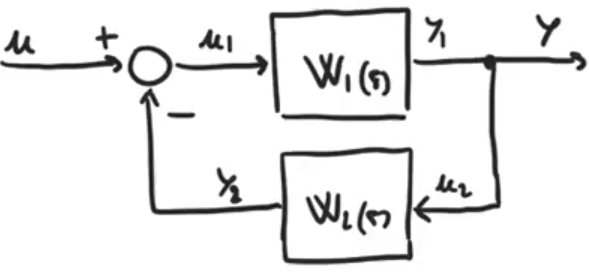
\includegraphics[width=\picwid]{blocchi_retroazione}
\end{figure}
$$
\begin{aligned}
S_1 &: \left\{\begin{aligned}
\dot{x}_1 & = A_1x_1 + B_1u_1\\
y_1 &= C_1 x_1
\end{aligned}\right. \\
S_2 & : \left\{\begin{aligned}
\dot{x}_2 & = A_2x_2 + B_2u_2\\
y_2 &= C_2 x_2
\end{aligned}\right. \\
\text{Vincoli} &: \left\{\begin{aligned}
y&=y_1=u_2\\
u_1 &= u -y_2
\end{aligned}\right.
\end{aligned}
$$
Aggregando gli stati
$$
\left\{\begin{aligned}
\dot{x}_1 & = A_1x_1 + B_1(u-C_2x_2)\\
\dot{x}_2 &= A_2x_2 + B_2(C_1x_1) \\
y &= C_1x_1
\end{aligned}\right.
$$
In forma compatta
$$
\left\{\begin{array}{cccc}
\dot{x}_1 =& \begin{pmatrix}
A_1 & -B_1C_2 \\ B_2C_1 & A_2
\end{pmatrix}x& +& \begin{pmatrix}
B_1 \\ 0
\end{pmatrix}u\\ \\
y =& \begin{pmatrix}
C_1 & 0
\end{pmatrix}x
\end{array}\right.
$$

La matrice $A$ non ha alcuna struttura particolare, dunque in generale gli
autovalori non hanno nulla a che fare con gli autovalori delle matrici $A_1$ e
$A_2$. Potrebbe anche accadere che il collegamento in retroazione di due
sistemi asintoticamente stabili generi un sistema instabile, viceversa due
sistemi instabili potrebbero diventare stabili, la retroazione è l'unica
connessione che modifica gli autovalori.
È l'unica soluzione che permette di stabilizzare un sistema inizialmente
instabile.

La funzione di trasferimento complessiva
$$
W(s) = \frac{N_1(s) D_2(s)}{D_1(s)D_2(s)+N_1(s)N_2(s)}
$$
Potrebbero esserci delle cancellazioni se $N_1$ e $D_2$ avessero divisori in
comune, uno zero del blocco di andata cancella un polo del blocco in ritorno,
si ottiene una parte del sistema contemporaneamente non raggiungibile e non
osservabile.
Se i termini in comune sono invece tra $D_1$ ed $N_2$ non si cancella nulla ma
il corrispondente autovalore non viene alterato dalla retroazione.
